% Reviewed solution for CritPt Challenge 57. Compiles with the supplied main.tex (natbib) and, through the
% fallbacks below, also with the original main.tex of the challenge package. Needs refs.bib, figs/ and template.py.
\providecommand{\citep}[2][]{\cite{#2}}
\providecommand{\citet}[2][]{\cite{#2}}
\providecommand{\citealt}[2][]{\cite{#2}}
\providecommand{\nat}{Nature}
\providecommand{\prl}{Physical Review Letters}
\providecommand{\prd}{Physical Review D}
\providecommand{\pra}{Physical Review A}

{\color{blue}\textbf{Reviewer's note.} The AI-generated solution has been replaced in full by the solution below, which was derived independently before the AI text was read, as the evaluation instructions suggest. The final answer follows the solution. An item-by-item assessment of the challenge statement, of the AI-generated solution and of its numerical script, with the AI text and script reproduced verbatim, follows the final answer in the accompanying document.}

\subsubsection*{Solution}

\paragraph*{Overview, conventions, and reproducibility}
The solution is provided in the following steps:
%
\begin{enumerate}[label=Step~\arabic*:,leftmargin=*,align=left,labelsep=0.5em,parsep=0pt,itemsep=0.1em,topsep=0.2em]
    \item The vector dark-matter field and its dark electric field are obtained from the dark-matter density.
    \item The $B-L$ coupling turns the dark electric field into a force on each mirror, and the free-mass response gives its displacement.
    \item The exact round trip of the laser light in one arm, with different charge-to-mass ratios for the inner and outer mirror, gives the change of the arm's optical path.
    \item The Michelson output is averaged over the unknown polarization and propagation direction of the field.
    \item The finite coherence of the field fixes the detection threshold for a $13$~yr observation.
    \item The smallest detectable $\epsilon_{B-L}$ follows for each $\delta q$.
\end{enumerate}
%
Throughout, $L$ is the arm length, $\sqrt{S_h}=3\times10^{-24}\,\mathrm{Hz}^{-1/2}$ the one-sided strain amplitude spectral density at $f=\omega/2\pi=250\,\mathrm{Hz}$, $T=13$~yr the observation time, $q_0=0.5$ the dark charge-to-mass ratio of the inner mirrors in units of $1/m_n$, $\delta q\in\{0.074,\,6\times10^{-3},\,5\times10^{-4}\}$ the excess of the outer mirrors, $m_n$ the neutron mass, and $e$ the elementary charge. Three conventions are fixed up front. (i) All quantities are evaluated in SI units with $\epsilon_0$ explicit, so that $\epsilon_{B-L}$, which is dimensionless, does not depend on the choice between Gaussian and Heaviside-Lorentz natural units made in the source literature.\footnote{\citet{Pierce2018} use $\hbar=c=\sqrt{4\pi\epsilon_0}=1$ and \citet{Morisaki2021} use $\hbar=c=\epsilon_0=1$. The force $\epsilon eQ_DE_D$ is the same physical quantity in both once the field amplitude is expressed through the energy density in the same units.} (ii) The strain sensitivity is a one-sided amplitude spectral density. (iii) $13$~yr means $13$ Julian years, $4.1025\times10^{8}$~s.

Every number below is produced by \texttt{challenge57.py}, which lists all problem inputs and all model inputs (with their sources) at its top, uses \texttt{astropy} (CODATA~2018) for physical constants, and prints its internal consistency checks under a \texttt{--verbose} flag. The problem does not state the dark-matter density, the dark-matter velocity, or the arm length. The values adopted for them are model inputs, chosen and justified in Steps~1, 3, and 5, and their consequences are reported in Table~\ref{tab:results}.

\paragraph*{Step 1: The vector field and its dark electric field}
A massive vector field of mass $m_A$ that makes up the dark matter is a superposition of nonrelativistic waves,
%
\begin{equation}
\mathbf A(t,\mathbf r)=\sum_i A_i\,\hat{\mathbf e}_i\cos(\omega_it-\mathbf k_i\cdot\mathbf r+\varphi_i),\qquad \omega_i\simeq\frac{m_Ac^2}{\hbar},\qquad \mathbf k_i=\frac{m_A\mathbf v_i}{\hbar},
\label{eq:field}
\end{equation}
%
where $A_i$, $\hat{\mathbf e}_i$, $\mathbf v_i$ and $\varphi_i$ are the amplitude, polarization unit vector, velocity and phase of the $i$-th wave \citep{Pierce2018,Morisaki2021}. At $f=250\,\mathrm{Hz}$, $m_Ac^2=hf=1.0339\times10^{-12}\,\mathrm{eV}$. Over one coherence time (Step~5) the sum acts as a single wave of amplitude $A_0$ with $\rho=\tfrac12m_A^2A_0^2$ in natural units, and the dark electric field $\mathbf E_D=-\partial_t\mathbf A$ has amplitude $m_AA_0=\sqrt{2\rho}$, independent of $m_A$. In SI units
%
\begin{equation}
E_D=\sqrt{\frac{2\rho}{\epsilon_0}} .
\label{eq:ED}
\end{equation}
%
The problem prompt does not explicitly provide $\rho$; we instead adopt $\rho=0.4\,\mathrm{GeV\,cm^{-3}}$ as given in Challenge~56, which is also the value commonly quoted in interferometer dark-photon analyses \citep{Pierce2018,Guo2019,Morisaki2021}. This choice gives $E_D=3804.8\,\mathrm{V\,m^{-1}}$.\footnote{The direct-detection convention is $\rho=0.3\,\mathrm{GeV\,cm^{-3}}$ \citep{LewinSmith1996,Baxter2021}. Since $\epsilon_{B-L,\min}\propto\rho^{-1/2}$, that choice raises every answer by $15\%$ (Table~\ref{tab:results}). The amplitude in any one coherence patch is Rayleigh distributed about the value implied by $\rho$ \citep{Centers2021}. Over the $\sim6\times10^{4}$ coherence times of a $13$~yr observation this averages out.}

\paragraph*{Step 2: Force on a mirror and its displacement}
The interaction $\mathcal L\supset-\epsilon_{B-L}\,e\,J^\mu_{B-L}A_\mu$ produces, in the nonrelativistic limit, a force $\mathbf F=\epsilon_{B-L}eQ_D\mathbf E_D$ on a body of $B-L$ charge $Q_D$, while the magnetic counterpart is suppressed by $v/c$ \citep{Pierce2018}. For a neutral atom the $B-L$ charge is its neutron number, so $Q_D/M=(A-Z)/(\mu\,m_n)$ with $A$, $Z$ and $\mu$ the mass number, atomic number and atomic mass in atomic units. This is $0.501/m_n$ for fused silica and $0.51/m_n$ for sapphire \citep{Michimura2020}, as follows from the standard atomic weights \citep{Prohaska2022}, and the problem's $q_0/m_n=0.5/m_n$ for the inner mirrors is the value for the fused-silica test masses of Advanced LIGO \citep{Aasi2015}. At $250\,\mathrm{Hz}$, far above the pendulum resonance of its suspension, a mirror responds to the force as a free mass, so its displacement along the polarization is
%
\begin{equation}
\delta x(t)=\frac{a}{\omega^2}\sin(\omega t-\mathbf k\cdot\mathbf r+\varphi),\qquad a=\epsilon_{B-L}\,e\,\frac{Q_D}{M}\,E_D .
\label{eq:dx}
\end{equation}
%
Per unit $\epsilon_{B-L}$ the inner mirrors have $e\,q_0/m_n=4.7828\times10^{7}\,\mathrm{C\,kg^{-1}}$, $a_0=1.8197\times10^{11}\,\mathrm{m\,s^{-2}}$ and $\delta x_0=a_0/\omega^2=7.3751\times10^{4}\,\mathrm{m}$. The outer mirrors have these multiplied by $(q_0+\delta q)/q_0$.

\paragraph*{Step 3: Exact round trip in one arm with a doped outer mirror}
Let the inner (input) and outer (end) mirrors of an arm along the unit vector $\hat{\mathbf n}$ sit at $x_i(t)=\hat{\mathbf n}\cdot\delta\mathbf x_i(t)$ and $x_e(t)=L+\hat{\mathbf n}\cdot\delta\mathbf x_e(t)$. Light leaving the inner mirror at $t-2L/c$ reflects from the outer mirror at $t-L/c$ and returns at $t$, so the round-trip path is \citep[Eq.~11]{Morisaki2021}, \citep[Eq.~9]{Michimura2020}
%
\begin{equation}
c\,T_r(t)=-x_i(t)+2x_e(t-L/c)-x_i(t-2L/c).
\label{eq:roundtrip}
\end{equation}
%
With $\delta\mathbf x_e=(1+\delta q/q_0)\,\delta\mathbf x$ evaluated at the outer mirror and $\delta\mathbf x_i=\delta\mathbf x$ at the inner mirror, and $\delta\mathbf x(t)\propto\sin\omega t$, the second difference of the common part gives $-\sin\omega t+2\sin\omega(t-L/c)-\sin\omega(t-2L/c)=4\sin^2(\omega L/2c)\,\sin\omega(t-L/c)$, so the change of the round-trip path is
%
\begin{equation}
\delta L(t)=\Big[\underbrace{4\sin^2\!\Big(\frac{\omega L}{2c}\Big)}_{\text{light-travel time}}+\underbrace{\frac{2\,\delta q}{q_0}}_{\text{doping}}\Big]\,\hat{\mathbf n}\cdot\delta\mathbf x(t-L/c)\;+\;\underbrace{2L\,(\hat{\mathbf n}\cdot\mathbf k)\,(\hat{\mathbf n}\cdot\delta\mathbf x_0)\cos\omega(t-L/c)}_{\text{field gradient}} .
\label{eq:dL}
\end{equation}
%
The light-travel-time term is the default signal, present without any doping. Because the light samples the two co-moving mirrors at times $2L/c$ apart, the optical path changes even though their separation does not \citep{Morisaki2021}. It is the second finite difference in time of the common displacement, $-x(t)+2x(t-L/c)-x(t-2L/c)$, which, for the sinusoidal mirror motion $\delta x\propto\sin\omega t$ driven by the field, equals $4\sin^2(\omega L/2c)\,\delta x(t-L/c)\approx(\omega L/c)^2\,\delta x$ and is therefore second order in $\omega L/c$. The doping term is the differential force introduced by the doping. The two terms oscillate in phase and therefore add constructively. Lastly, the field-gradient term is the phase difference of the field across the arm, the original signal of \citet{Pierce2018}, in quadrature with the others and suppressed by $kL=m_AvL/\hbar$. With $L=3994.5\,\mathrm{m}$ \citep{Aasi2015},\footnote{The problem says only ``LIGO''. Using the nominal $4000$~m instead changes the answers by $0.13\%$ (Table~\ref{tab:results}).} $\omega L/c=2.0930\times10^{-2}$, $4\sin^2(\omega L/2c)=4.380\times10^{-4}$, $2\delta q/q_0=0.296,\ 0.024,\ 0.002$, and $2kL=3.21\times10^{-5}$ for $v=230\,\mathrm{km\,s^{-1}}$ (Step~5). The undoped light-travel-time term is thus $0.15\%$, $1.8\%$ and $22\%$ of the doping term for the three values of $\delta q$: never dominant, but not negligible at the precision requested, and for the smallest $\delta q$ it changes the answer by a fifth (Fig.~\ref{fig:ltt}).

\begin{figure}[t]
\centering
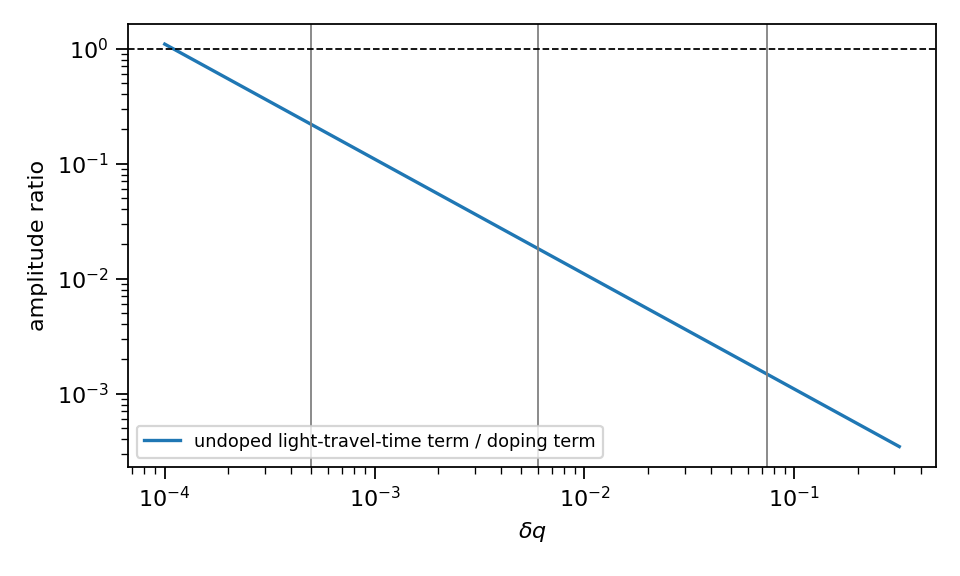
\includegraphics[width=0.6\linewidth]{figs/ltt_vs_doping.png}
\caption{Ratio of the undoped light-travel-time term to the doping term in Eq.~\eqref{eq:dL} as a function of $\delta q$ at $250$~Hz and $L=3994.5$~m. Vertical lines mark the three values of $\delta q$ in the problem. The dashed line marks equality, reached only at $\delta q=1.1\times10^{-4}$.}
\label{fig:ltt}
\end{figure}

\paragraph*{Step 4: Michelson output averaged over the field orientation}
The detector output is $h(t)=-[\delta L_{\hat{\mathbf n}}(t)-\delta L_{\hat{\mathbf m}}(t)]/(2L)$ for arms along $\hat{\mathbf n}$ and $\hat{\mathbf m}$ with $\hat{\mathbf n}\cdot\hat{\mathbf m}=0$ \citep[Eq.~9]{Morisaki2021}. The Fabry-Perot arm cavities amplify any change of the arm length, and that amplification is already contained in the strain sensitivity \citep{Morisaki2021}. The polarization and propagation direction of the field are unknown and, over $13$~yr, are sampled through the rotation of the Earth, so the relevant quantity is the mean square over an isotropic distribution of $\hat{\mathbf e}$ and $\hat{\mathbf k}$, with $\langle(\hat{\mathbf n}\cdot\hat{\mathbf e})^2\rangle=1/3$ and no correlation between $\hat{\mathbf e}$ and $\hat{\mathbf k}$ \citep{Pierce2018,Morisaki2021,Michimura2020}.\footnote{Two distinct averages are involved, over the propagation direction $\hat{\mathbf k}$ and over the polarization $\hat{\mathbf e}$. Neither is isotropic by kinematics alone: the halo wind is ordered and the velocity ellipsoid of a virialized halo is anisotropic, and the Earth's rotation does not randomize a fixed $\hat{\mathbf e}$. The average over $\hat{\mathbf k}$ is nevertheless irrelevant at the precision requested, since $\hat{\mathbf k}$ enters only the field-gradient term, below $10^{-4}$ of the signal here. The average over $\hat{\mathbf e}$ is a genuine assumption about the field, that its polarization is randomized between the $\sim6\times10^{4}$ coherence patches sampled in $13$~yr. It is the convention under which all published limits are quoted \citep{Pierce2018,Morisaki2021,LVK2022}, and \citet{Michimura2020} note that a production mechanism leaving only longitudinal or only transverse modes would violate it. Its exposure is $\mathcal O(1)$: the in-phase amplitude scales as $|(\hat{\mathbf n}-\hat{\mathbf m})\cdot\hat{\mathbf e}|$, whose isotropic root mean square $\sqrt{2/3}$ would become $\sqrt2$ for a fixed polarization along $\hat{\mathbf n}-\hat{\mathbf m}$ and $0$ for one normal to the detector plane.} Writing $\Gamma\equiv4\sin^2(\omega L/2c)+2\delta q/q_0$ and averaging Eq.~\eqref{eq:dL} over time and orientation,
%
\begin{equation}
\langle h^2\rangle=\frac{\delta x_0^2}{4L^2}\left[\frac{\Gamma^2}{3}+\frac{(2kL)^2}{9}\right]\epsilon_{B-L}^2 .
\label{eq:h2}
\end{equation}
%
For $\delta q=0$ this reproduces Eqs.~(23) and (24) of \citet{Morisaki2021} exactly, fixing the averaging factors independently of our derivation. Per unit $\epsilon_{B-L}$, $\langle h^2\rangle^{1/2}=1.5800$, $0.13025$ and $0.012995$ for the three values of $\delta q$. The field-gradient term has a relative contribution $\leq10^{-4}$ in all three cases.

\paragraph*{Step 5: Detection threshold for a $13$~yr observation}
The field is coherent only over $\tau=2\pi/(m_Av^2)$, the time over which waves differing by the local dark-matter velocity dispersion $v$ (the notation of the source literature) dephase \citep[Eq.~5]{Morisaki2021}. The problem does not give $v$. We adopt $v=230\,\mathrm{km\,s^{-1}}$ as provided in the Challenge~56 prompt, which is also the value commonly adopted in the literature \citep{Pierce2018,Morisaki2021,Michimura2020}. This gives $\tau=6796$~s, so the $13$~yr observation spans $T/\tau=6.0\times10^{4}$ coherence times.\footnote{As in any wave-like dark-matter search, the line shape depends on two velocities, the dispersion of the halo and the streaming speed of the detector through it, and $230\,\mathrm{km\,s^{-1}}$ is the galactic rotation speed of the classic halo model \citep{LewinSmith1996}. The source papers use it in both roles, as do we.} Beyond one coherence time the phase of the field becomes stochastic, so the signal cannot be integrated coherently over the full $T$. The appropriate search instead sums the power of successive Fourier transforms of length $\sim\tau$ \citep{Miller2021,LVK2022}. The sensitivity still improves with observation time, but only as $T^{1/4}$ in amplitude rather than the $T^{1/2}$ of a coherent signal, because the powers of the $N=T/\tau$ independent stretches add with $\sqrt N$ fluctuations. The resulting detection threshold is \citep[Eqs.~20 and 21]{Morisaki2021}, \citep[Eq.~9]{Pierce2018}
%
\begin{equation}
\langle h^2\rangle_{\rm thr}=\frac{S_h(f)}{T_{\rm eff}},\qquad T_{\rm eff}=\sqrt{\tau T}=1.6697\times10^{6}\,\mathrm{s},\qquad \langle h^2\rangle_{\rm thr}^{1/2}=2.3217\times10^{-27},
\label{eq:thr}
\end{equation}
%
which is the statement that the signal power equals the noise power in the power statistic, i.e., a power signal-to-noise ratio of one. We adopt this as the meaning of ``SNR~$=1$'' because it is the convention of the literature the problem is built on.\footnote{It is not the only possible reading. In Challenge~56 we defined SNR through the amplitude matched filter, $h_0\sqrt{T/S_h}=1$ for a monochromatic signal, and carried the finite coherence through the exact factor $R(T)$ derived from the field correlation function of \citet{Derevianko2018}. With $\langle h^2\rangle=h_0^2/2$ that convention gives $R(T)=20.28$ here and thresholds $8.5\%$ lower (Table~\ref{tab:results}). The two differ by $\mathcal O(1)$ factors inherent to defining an SNR for a stochastic signal, and the problem statement does not choose between them.}

\paragraph*{Step 6: The coupling detection threshold}
Combining Eqs.~\eqref{eq:h2} and \eqref{eq:thr},
%
\begin{equation}
\epsilon_{B-L,\min}=\left[\frac{S_h/T_{\rm eff}}{\langle h^2\rangle/\epsilon_{B-L}^2}\right]^{1/2}
=1.47\times10^{-27},\quad 1.78\times10^{-26},\quad 1.79\times10^{-25}
\label{eq:final}
\end{equation}
%
for $\delta q=0.074$, $6\times10^{-3}$ and $5\times10^{-4}$. Table~\ref{tab:results} shows how the forecast thresholds vary under the alternative assumptions discussed above. For scale, the same formula with no doping at all gives $\epsilon_{B-L,\min}\approx1\times10^{-24}$ for $13$~yr, the undoped reach of \citet{Morisaki2021} extended in time. The doping improves it by $2\delta q/q_0$ divided by $4.4\times10^{-4}$.

\begin{table}[t]
\centering
\caption{Smallest detectable $\epsilon_{B-L}$ at $250$~Hz, $T=13$~yr, for the three values of $\delta q$. ``Exact'' is Eq.~\eqref{eq:dL} with all three terms, $L=3994.5$~m, $\rho=0.4\,\mathrm{GeV\,cm^{-3}}$, $v=230\,\mathrm{km\,s^{-1}}$, and the power threshold of Eq.~\eqref{eq:thr}.}
\label{tab:results}
\small
\begin{adjustbox}{max width=\linewidth}
\begin{tabular}{llccc}
\toprule
signal model & threshold & $\delta q=0.074$ & $6\times10^{-3}$ & $5\times10^{-4}$ \\
\midrule
exact (this work) & Eq.~\eqref{eq:thr} & $1.47\times10^{-27}$ & $1.78\times10^{-26}$ & $1.79\times10^{-25}$ \\
doping term only (as the problem implies) & Eq.~\eqref{eq:thr} & $1.47\times10^{-27}$ & $1.82\times10^{-26}$ & $2.18\times10^{-25}$ \\
exact & amplitude matched filter, $R(T)$ & $1.34\times10^{-27}$ & $1.63\times10^{-26}$ & $1.63\times10^{-25}$ \\
exact, $L=4000$~m & Eq.~\eqref{eq:thr} & $1.47\times10^{-27}$ & $1.78\times10^{-26}$ & $1.79\times10^{-25}$ \\
exact, $\rho=0.3\,\mathrm{GeV\,cm^{-3}}$ & Eq.~\eqref{eq:thr} & $1.70\times10^{-27}$ & $2.06\times10^{-26}$ & $2.06\times10^{-25}$ \\
\bottomrule
\end{tabular}
\end{adjustbox}
\end{table}

\paragraph*{What the problem idealizes}
(i) \emph{The undoped signal.} The problem attributes the differential force to the doping alone. The finite light-travel time produces a differential signal even for identical mirrors, in phase with the doping term. It is included in the primary answer and is what separates the first two rows of Table~\ref{tab:results}. (ii) \emph{Realizability of $\delta q$.} The $B-L$ charge-to-mass ratios of the usual optics differ by about $0.01$ (silica $0.501$, sapphire $0.51$; \citealt{Michimura2020}), so $\delta q=6\times10^{-3}$ is a silica-versus-sapphire-scale difference and $5\times10^{-4}$ an isotopic-doping level, whereas $\delta q=0.074$ would require a mirror substrate of a heavy element such as indium, cadmium or tin, whose neutron fractions $(A-Z)/\mu$ computed from the standard atomic weights \citep{Prohaska2022} are $0.57$ to $0.58$, not a dopant. (iii) \emph{Provenance.} To our knowledge the configuration has not been proposed in the published literature. The closest precedents are the composition dipoles of equivalence-principle tests, mirrors of different thickness proposed for scalar dark matter \citep{GroteStadnik2019}, the different response of KAGRA's sapphire test masses and fused-silica auxiliary mirrors exploited through auxiliary length channels \citep{Michimura2020}, and the use of different materials in an optomechanical accelerometer \citep{Manley2021}. It is a natural extension of these, and nothing in the calculation depends on its provenance; we just flag this for assessment completeness. (iv) \emph{Thirteen years of continuous data.} The threshold of Eq.~\eqref{eq:thr} assumes $13$~yr of uninterrupted data at a constant sensitivity, whereas real detectors have duty cycles (the fraction of calendar time spent taking science data) well below $100\%$ and are upgraded between observing runs, so that the sensitivity improves over such a span. It also treats $v$ as constant, although the Earth's orbital motion modulates the lab-frame speed by about $\pm15\,\mathrm{km\,s^{-1}}$ over the year, the component of the $30\,\mathrm{km\,s^{-1}}$ orbital velocity along the halo wind \citep[Eq.~3.6]{LewinSmith1996}, and hence $\tau$ by about $\pm13\%$, and it uses the mean-square field amplitude, although the amplitude fluctuates from one coherence patch to the next. Both effects average over the $6\times10^{4}$ coherence patches of the observation.

\paragraph*{Is the problem well posed?}
As a statement it is: the requested quantity is defined for each $\delta q$. It is not closed in its inputs: the dark-matter density, the dark-matter velocity (which sets the coherence time and hence $\epsilon_{\min}\propto v^{1/2}$) and the arm length are not given and must be supplied externally, here inherited from the Challenge~56 prompt ($\rho$, $v$) or taken from the instrument literature ($L$), and the mirror material is only implied by $q_0=0.5$. Nor is it closed in its conventions: ``SNR~$=1$'' for a stochastic, incoherently summed signal is a power statistic in the problem's source literature but an amplitude statistic in others, an $\mathcal O(1)$ difference ($8.5\%$ here). The statement also omits one piece of physics, the undoped light-travel-time signal of Step~3. It raises the signal by $0.15\%$ and $1.8\%$ for the two larger $\delta q$ but by $22\%$ for the smallest, for which the answer is lowered by $18\%$. At three significant digits the answers therefore depend on these choices. The exact chain above states each one and Table~\ref{tab:results} quantifies each. Agreement with a reference answer beyond the second digit would test which conventions the reference adopted, not the physics.

\paragraph*{Filled \texttt{template.py}}
\lstinputlisting[style=answerstyle,caption={\texttt{template.py}}]{template.py}

\bibliographystyle{unsrtnat}
\bibliography{refs}
